\chapter{Estado del arte}

En este capítulo se realizará una revisión de documentación y literatura sobre los siguientes enumerados a continuación, que se consideraron relevantes para una comprensión sólida del proyecto a realizar.

[CAMBIAR ORDEN DE ITEMS]
\begin{itemize}
    \item \textbf{Motores de videojuegos}: Este trabajo ya tiene como premisa el uso de \textit{Godot} como motor. Sin embargo es relevante estudiar y comparar los principales motores de mercado, sus especificaciones técnicas, filosofía, precio y modelo de negocio. Así se podrá justificar la que es una de las decisiones más importantes a la hora de emprender un desarrollo.
    
    \item \textbf{Género Metroidvania}: Antes de planear un videojuego es importante realizar un estudio de mercado previo para hacerse una idea de cual es el alcance comercial esperado de uno. Un tipo de juego poco demandado o saturado en el mercado aumenta mucho el riesgo de resultar en un proyecto no rentable. Además es necesario estudiar otras propuestas similares e identificar cuales son sus características, tropos y qué suele buscar el público en ellos. Se añadirá en esta sección una brevísima revisión a la historia y características del género para el lector que esté interesado.
    
    \item \textbf{Características y retos del desarrollo de videojuegos}: [REVISAR ESTE FRAGMENTO] Se estudiarán las distintas propuestas y enfoques de metodologías existentes, poniendo especial interés en casos los reales y testimonios de veteranos de la industria. Se identificarán las carencias y problemas de las propuestas existentes, así como los problemas más comunes. La síntesis de este apartado será crucial para el capítulo de planificación.
    
    \item \textbf{Arquitecturas y patrones}: Revisión de las principales arquitecturas de proyectos de videojuegos en general y las prácticas comunes de Godot en específico.
    
    \item \textbf{Opciones de accesibilidad}: Estas opciones se proponen adaptar las experiencias jugables desde distintos enfoques para que personas con distintas preferencias, dificultades psicomotrices, nivel de habilidad o edad puedan disfrutar de los videojuegos. Lamentablemente, a día de hoy no todos los juegos cuentan con opciones de este tipo pese a su importancia, ya que permiten ampliar el público potencial. Se estudiarán cuales son las principales dificultades con la que se puede encontrar una persona, qué soluciones existen y cuales se pueden aplicar al proyecto.
    
    \item \textbf{Videojuegos como software libre}: Se estudiará el uso de software libre como forma de distribución y modelo de negocio para videojuegos. [IGUAL NO APLICA]
    
    \item \textbf{Herramientas para testing y QA}: Se investigarán las distintas herramientas para la realización de test y, en general, garantizar la calidad software en videojuegos y en Godot.

\end{itemize} 

Tras esta investigación se pretende tener una visión de conjunto sobre estos campos. Es crucial adquirir esta visión antes de planificar y comenzar el proyecto, pues permitirán tomar decisiones informadas en temas muy determinantes a largo plazo y con potencial impacto en la calidad y rédito económico del producto resultante.


[REVISAR ESTA PARTE]


Para la búsqueda de información se usó principalmente búsquedas en internet y en repositorios como Google Scholar, Scopus y la biblioteca de la Universidad de Granada.

Se consultarán sobre las distintas herramientas software sus páginas oficiales de documentación, términos de uso, contratos y licencias. También se estudiarán las publicaciones científicas disponibles sobre los temas a abordar. Debido a que al panorama científico aplicado al desarrollo de videojuegos le queda mucho por desarrollar, se prestará atención a los distintos testimonios y ponencias de los profesionales de la industria que hayan explicado cómo funcionan en su equipo, cómo enfocan un desarrollo y qué prácticas encuentran más efectivas. Las ponencias en eventos profesionales como la \textit{GDC (Game Developer Conference)} o \textit{Guadalindie} pueden ser muy útiles.

\section{Motores de videojuegos}

Existe una gran variedad de motores de videojuegos. Algunos de ellos tienden a ser más generalistas, y otros se especializan en nichos como \textit{Ren'Py}\cite{renpy}, el cual está enfocado al desarrollo de novelas visuales. Algunos de los motores más relevantes en el mercado actual como \textit{RE Engine} o \textit{Frostbite} son software privado usado por sus empresas propietarias para desarrollos internos, por lo que el público general no tiene acceso a ellos. Tomando de referencia \textit{The Big Game Engine Report of 2025}\cite{game-engine-report} y cribando las opciones de nichos y privadas, los motores accesibles más relevantes en lanzamientos de 2024 fueron los siguientes:

\begin{itemize}
    \item Unreal Engine
    \item Unity
    \item GameMaker
    \item Godot Engine
\end{itemize}

\subsection{GameMaker}

GameMaker\cite{gamemaker} es un motor enfocado al desarrollo de juegos 2D. No tiene capacidad de trabajar con gráficos 3D. Desde su web oficial se anuncian como un motor indicado para primerizos en el desarrollo de videojuegos y programación en general, pero apuntando también cómo muchos equipos profesionales que trabajan en proyectos grandes siguen apostando por el. Las claves de su accesibilidad se debe a varios factores; Su lenguaje de programación, \textit{GML}, cuenta con un editor gráfico sencillo que funciona con nodos y etiquetas. La interfaz general del motor cuenta con muchos elementos \textit{drag and drop}. Cuenta con un editor de \textit{habitaciones} con el que se pueden dibujar fácilmente instancias del juego.

Además, la arquitectura de los proyectos y los cauces de trabajo que promueve el motor son ideales para acelerar el proceso de creación de la mayoría de los juegos 2D. Es interesante apuntar que al tratarse de un motor muy popular, en internet se pueden encontrar fácilmente muchos recursos, tutoriales y foros para poder solventar cualquier problema que se tenga durante el desarrollo.

El motor tiene soporte multiplataforma y permite exportar proyectos a todas las plataformas principales de videojuegos (Windows, Linux, Mac, Playstation, XBOX, Nintendo Switch y smartphones).

En cuanto a su modelo de negocio, GameMaker presenta tres opciones:

\begin{itemize}
    \item \textbf{Uso gratuito}: Permite usar el motor en todas sus capacidades pero no permite el uso comercial de los videojuegos creados. Permite exportar los mismos a escritorio, web o móvil.
    \item \textbf{Profesional}: Se accede a través de un pago único. Es similar al uso gratuito con la excepción de se permite el uso comercial de los juegos.
    \item \textbf{Enterprise}: Se accede a través de una suscripción mensual o anual. Permite exportar al resto de plataformas y da acceso al código fuente de GameMaker. La licencia con la que se permite el acceso al código permite únicamente ver, usar, copiar, modificar, extender o alterarlo con el único propósito de depurar u optimizar el producto creado a través del software. No permite aplicar una sublicencia o cualquier uso comercial sobre el código.
\end{itemize}

En resumen, GameMaker es un motor recomendado para hacer videojuegos 2D. Tiene formas de trabajar propias pero son presuntamente eficaces para la construcción de ese tipo de juegos. Cuenta con opciones gratis y de pago en función del alcance comercial deseado. No es software libre.

\subsection{Unity}

Unity\cite{Unity} ha sido en los últimos años el motor más popular entre desarrolladores independientes además de ocupar un cuarto\cite{game-engine-report} de la cuota de mercado de \textit{Steam}. Permite la construcción de videojuegos tanto 2D como 3D, aunque destaca más por estos últimos. Puede exportar para web, consolas, móviles, gafas de \textit{realidad virtual} entre otros. Emplea C\# como lenguaje de programación.

Dependiendo de el plan elegido, el motor cuenta también con distintos servicios satélite y herramientas enfocadas a facilitar el desarrollo, como un motor especializado de físicas, herramientas de red para crear juegos \textit{online}, un \textit{asset manager} con una tienda de recursos incluida, herramientas de diagnóstico de errores, o líneas para soporte y aprendizaje. Estas características están repartidas en 4 niveles de suscripción, siendo la primera de ellas gratis y el resto por cobro mensual. Independientemente de sus características, todas ellas tienen una restricción\cite{unity-license} en función de los ingresos de la entidad que los use:

\begin{itemize}
    \item \textbf{Personal}: Para entusiastas y pequeños equipos. Permite el uso comercial mientras las ganancias totales de todos los productos bajo un titular no sobrepasen los \$200,000 USD en los últimos 12 meses.
    \item \textbf{Pro}: Para equipos o desarrolladores experimentados. Elegible unicamente si no se sobrepasan los \$24,999,999 USD en ganancias.
    \item \textbf{Enterprise}: Para grandes equipos y problemas complejos. Ofrece un kit completo de todas las funcionalidades y servicios de Unity enfocado a videojuegos.
    \item \textbf{Industry}: Para aplicaciones de tiempo real en 3D como formación de empleados, configuración de producto o sistemas embebidos.
\end{itemize}

Unity cuenta con recursos propios para aprender a manejar el motor. Además de eso y debido a su popularidad y activa comunidad hay muchos recursos de terceros.

Es importante mencionar una polémica\cite{unicty-scandal} ocurrida alrededor de Unity en años recientes. Se anunció un cambio en los términos y condiciones a través de los cuales todos los juegos que superaran los \$200,000 USD en facturación deberán pagar un impuesto adicional \textbf{por cada instalación} que los consumidores realizaran del juego, las cuales podrían ser de hasta 20 céntimos. Este cambio sentó mal en la comunidad de desarrolladores por considerarse abusiva. Tras algunas semanas de protestas, Unity decidió echarse atrás con este cambio. Pero esto destapa una debilidad de Unity (y otros motores privativos): el negocio que se pueda usando este motor está a merced de la empresa propietaria y sus políticas. Nada asegura que en un futuro no pueda volver a realizarse otro cambio similar en un futuro.

En resumen, Unity es un motor sólido y asentado en la industria, con muchos recursos online que puede cumplir su función si sus cuotas son asumibles, pero que cuenta con una dirección que ha dado pasos en falso y generado desconfianza en el futuro del proyecto. Huelga decir que no es software libre.

\subsection{Unreal Engine}

Unreal Engine en sus diferentes versiones (siendo Unreal Engine 5 la última) es el motor gráfico público más puntero tecnológicamente hablando. Está enfocado en la creación de juegos 3D, aunque también es posible hacerlos 2D. Emplea principalmente C++ como lenguaje de programación (considerado el estandar de la industria) aunque tiene opciones para poder usar otros como Python. El motor además es usado en múltiples sectores además de el del videojuego, como el cine o en experiencias de realidad virtual.

El motor cuenta con decenas de herramientas muy avanzadas tecnológicamentes para, entre otros, partículas físicas de ropa, físicas de pelo, sistema integrado de física de destrucción, infraestructura multijugador, diseñador de UI, nubes de puntos, herramientas de terreno, \textit{world partition} para facilitar crear mundos abiertos, generación de contenido procedural, físicas de agua, etc. Permite exportar a todas las plataformas actuales, con soporte de realidad aumentada.

Es un software muy potente enfocado al uso profesional, y por ello tiene una curva de aprendizaje más pronunciada, requiere conocimiento más técnico y de bajo nivel y se pueden encontrar bastantes menos recursos en internet comparado con otras opciones.

El uso de el motor íntegro es gratuito mientras no se superen unos ingresos de un millón de dólares. A partir de ese punto, es posible continuar de dos formas. O bien pagando el 5\% de los ingresos que generen los productos, o pagando una licencia por cada puesto de trabajo que dispongas. Para todas las licencias, incluida la gratuita, se tiene acceso al código fuente de Unreal Engine. Sin embargo no es software libre. Es necesario tener una cuenta de Unreal Engine con algún plan para acceder a el y su uso está sujeto a la licencia de \textit{Epic}, la empresa matriz.

En resumen, Unreal Engine es el motor público más puntero y potente en lo que a gráficos 3D se refieren. Tiene muchas herramientas para desarrollar productos profesionales sólidos siempre y cuando se cuente con el conocimiento técnico suficiente. Sus planes son relativamente generosos, permitiendo el uso comercial de pequeños desarrolladores sin muchas ganancias sin ahogarlos con licencias caras.

\subsection{Godot Engine}
%%

proyectos comerciales existentes

%%


La característica principal de Godot Engine\cite{godot} es que es \textit{FOSS (Free and Open Source Software)}. Su código está publicado en \textit{\href{https://github.com/godotengine/godot}{GitHub}} y cualquiera puede contribuir para mejorarlo. Está publicadobajo la licencia MIT, que permite modificación, distribución y uso comercial del software mientras se publique bajo la misma licencia.

\begin{figure}[h]
    \centering
    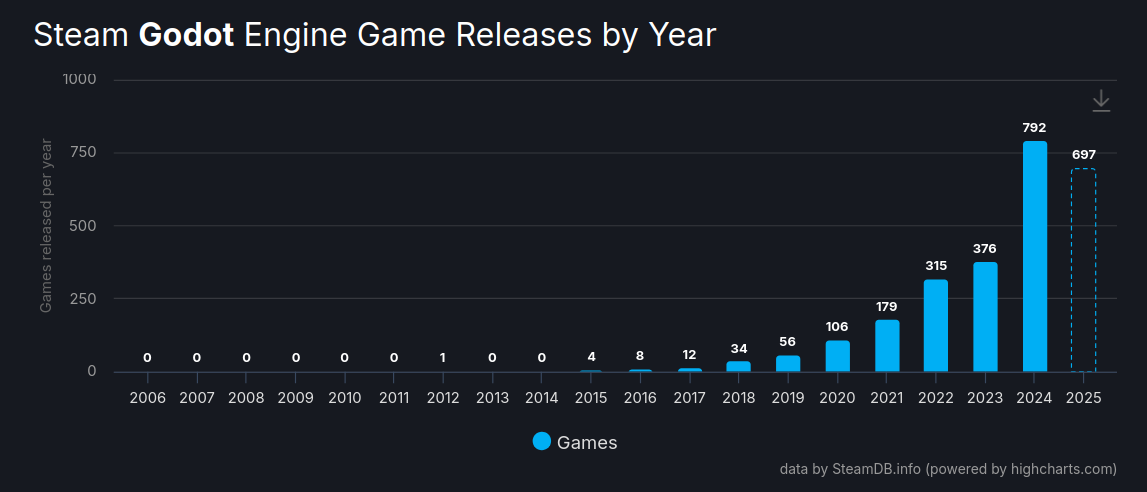
\includegraphics[scale=0.35]{img/godot-by-year.png}
    \caption[Juegos publicados en Godot por año]{Juegos desarrollados con Godot publicados en Steam por año según SteamDB\cite{steamdb}}
    \label{fig:godotbyyear}
\end{figure}

El motor está expresamente diseñado para creación de juegos 2D, 3D y de \textit{Extended Reality} (término paraguas que auna la realidad virtual y realidad aumentada entre otras). Puede exportar para web, Windows, MacOS, Linux y plataformas móviles. \textbf{No tiene soporte oficial para exportar a videoconsolas}\cite{godot-console-export}. Esto se debe a que las consolas son plataformas cerradas que requieren de leyes y acuerdos de confidencialidad estrictos incompatibles con su naturaleza de software libre. Aun así es posible exportar a consolas haciendo uso de herramientas de terceros. Como lenguage emplea GDScript\cite{gdscript}, un lenguage interpretado similar a Python desarrollado específicamente para las necesidades de Godot. También es posible emplear otros lenguajes como C\# y C++, este último siendo interesante para proyectos con necesidades técnicas más altas ya que cuenta con una mayor velocidad de ejecución.

Godot trabaja sobre un concepto fundamental: sus \textbf{Nodos}. Un nodo es un elemento que encapsula un nombre y propiedades mutables. Este recibe en cada instante señales que actualizan su estado. Son extensibles (en el mismo sentido por el que se entiende extender en el ámbito de la programación orientada a objetos) y a un nodo dado se le pueden añadir otros \textbf{nodos hijos}. De esta forma, una ejecución de un programa en Godot consta de una colección de nodos compuestos en forma de grafo árbol.

En la figura \ref{fig:godotsceneexpample} se puede observar como luce un ejemplo de un nodo \textit{Character}, que representa a un personaje, probablemente el del jugador. Este nodo está compuesto de otros nodos hijos que lo dotan de propiedades, como una imagen, una forma de colisión para sus físicas y una cámara que lo sigue y lo muestra por pantalla. En la figura \ref{fig:godottreeexpample} se puede ver un ejemplo de un proyecto sencillo. Todos los nodos cuelgan de la raíz del proyecto, \textit{Scene}. Contamos con un nodo \textit{Level}, conteniendo un nivel del juego, \textit{CanvasLayer} encargado de mostrar el decorado de fondo de dicho nivel, y un segundo \textit{CanvasLayer} en el que se muestra la interfaz de usuario.

\begin{figure}[h]
    \centering
    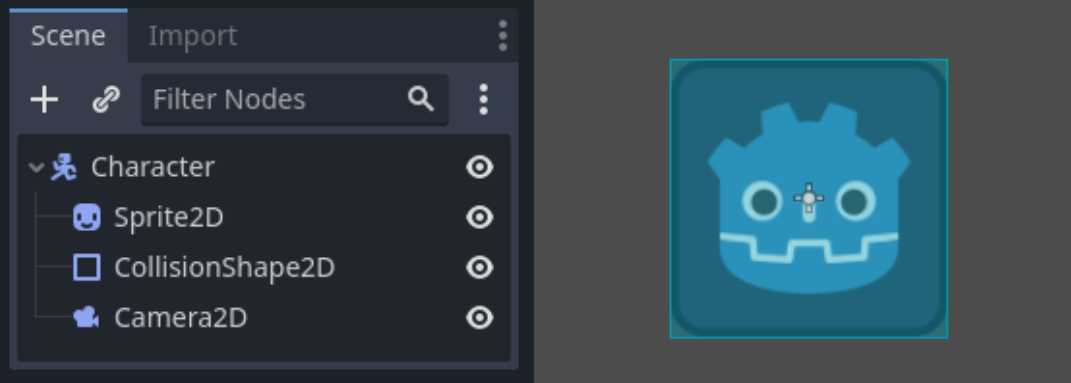
\includegraphics[scale=0.3]{img/godot-node.png}
    \caption[Ejemplo de escena de Godot]{Ejemplo de una escena 'Personaje' compuesta de nodos extraida de Godot Docs\cite{godot-docs}}
    \label{fig:godotsceneexpample}
\end{figure}

\begin{figure}[h]
    \centering
    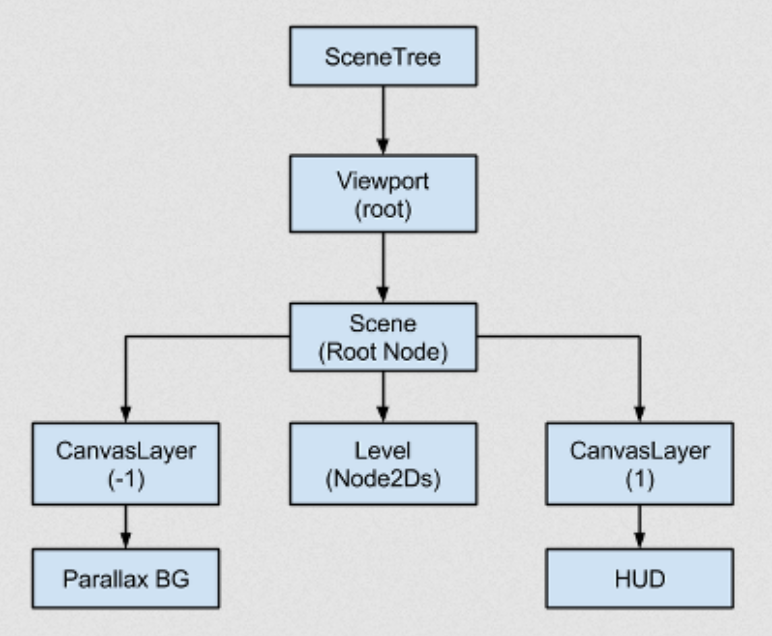
\includegraphics[scale=0.3]{img/godot-node-structure.png}
    \caption[Ejemplo de grafo de nodos en Godot]{Ejemplo de una organización en árbol de los nodos que componen un juego en Godot, extraido de Godot Docs\cite{godot-docs}}
    \label{fig:godottreeexpample}
\end{figure}

En 2014 Godot fue publicado y su código fue liberado. De esto fue responsable Okam Studio, estudio de videojuegos argentino que dejó de estar en activo en 2019. Durante más de 10 años, Godot fue desarrollado como motor privado para los proyectos del estudio, que finalmente decidió liberarlo. Lo que empezó siendo el proyecto de una empresa con dos trabajadores, en diciembre acabó acumulando aportaciones de más de 2800 usuarios en su repositorio. En la base de datos SteamBD\cite{steamdb} se puede consultar como ha ido creciendo el número de juegos publicados con Godot cada año. 2024 supuso una exlposión de casi el doble de publicaciones, llegando a 792.

En 2022 aparece de la mano de los dos fundadores \textit{Godot Foundation}\cite{godot-foundation}, organización sin ánimo de lucro que se dedica a gestionar en lo técnico y en lo económico el desarrollo del motor. Se financian enteramente a través de donaciones de usuarios y empresas patrocinadoras, entre las que se encuentran desarrolladoras de videojuegos que usan el motor, por lo que está en el mejor de sus intereses el desarrollo del proyecto. El código permanece abierto y recibiendo aportaciones de usuarios de todo el mundo, siendo la diferencia que, gracias a las donaciones, pueden permitirse contratar a ingenieros a tiempo completo para que gestionen y desarrollen el proyecto.

Es crucial remarcar la importancia de tener un proyecto de software libre tan ambicioso como el de Godot. Si bien es cierto que sus capacidades técnicas en cuanto a 3D no son ni de lejos tan punteras como las de Unity y mucho menos Unreal Engine, es muy probable que con el tiempo la brecha vaya menguando. En menos de un lustro, el proyecto ha crecido enormemente en todos los aspectos: usuarios, características y financiación. Esta tendencia parece mantenerse y, sumado a la robustez que confiere el software libre con una gran comunidad detrás, parece inteligente apostar por Godot en el largo plazo. Además, la licencia MIT da a los estudios grandes ventajas de forma inmediata. Recortan gastos en licencias y no están atados a ningún contrato que pueda cambiar en el futuro y comprometer su actividad comercial, como recientemente ocurrió con Unity.

Pese a lo relativamente novel que es el motor, ya cuenta con grandes proyectos 2D y 3D lanzados tanto para ordenador, móvil y videoconsolas. Aquí algunos: \href{https://www.nintendo.com/es-es/Juegos/Juegos-de-Nintendo-Switch/Sonic-Colours-Ultimate-2014880.html?srsltid=AfmBOopP2Gm2S3Zo5fcoc3Ifz5E1b136K8O_6Y2vLMouJm2Zj5LI0aut}{Sonic Colours Ultimate}, \href{https://store.steampowered.com/app/2868840/Slay_the_Spire_2/}{Slay the Spire 2}, \href{https://store.steampowered.com/app/2835570/Buckshot_Roulette/}{Buckshot Roullete}, \href{https://store.steampowered.com/app/1321440/Cassette_Beasts/}{Cassete Beast}, \href{https://store.steampowered.com/app/1677770/The_Case_of_the_Golden_Idol/}{The Case of the Golden Idol}, etc.

En resumen, Godot es ideal para construir juegos 2D y también 3D aunque con limitaciones. Su licencia y modelo de negocio son los más interesantes desde el punto de vista del cliente. Su sistema de nodos es muy potente de cara a construir la arquitectura de un proyecto. Y por último, su tendencia al alza promete mayor crecimiento en el medio y largo plazo.

\section{Características y retos del desarrollo de videojuegos}

\subsection{Diferencias entre el desarrollo de videojuegos y de software generalista}

Para comprender por qué el desarrollo de videojuegos debe ser objeto de estudio en si mismo, hay que analizar sus diferencias respecto a otros tipos de software. La publicación de Murphy-Hill et al.\cite{murphy-hill} proporciona una buena comprensión de partida para abordar el tema. Realizaron un estudio en el que se entrevistó y encuestó a desarrolladores de videojuegos, de software generalista, y otros con una experiencia en ambos sectores con el fin de analizar en qué se diferenciaban. Tras un análisis estadístico de las respuestas, el estudio concluía con cierto grado de certeza que:

\begin{enumerate}
    \item En videojuegos los requisitos son menos claros que en otro software.
    \item La creatividad se valora más en los equipos que desarrollan videojuegos.
    \item En videojuegos se valora más la habilidad de comunicarse con empleados no ingenieros.
    \item Los equipos que desarrollan videojuegos necesitan ser más diversos.
    \item En videojuegos, los desarrolladores tienden a usar lo que ellos perciben como metodologías Ágiles más que en otro software.
    \item El trabajo de desarrollador de videojuego recibe mayor admiración. 
\end{enumerate}

Se puede deducir que los puntos 1, 2, 3 y 4 están estrechamente relacionados con el hecho de que los videojuegos además de software son productos creativos y artísticos. Este aspecto puede explicarse desde dos prismas: el del \textit{requisito de diversión} y el de las disciplinas involucradas, que se explican a continuación.

El software generalista suele estar diseñado como una herramienta que cumple un propósito, por tanto es relativamente fácil requisitar qué puntos o necesidades debe cubrir. En contraste, el fin último de un VJ es entretener de alguna forma al usuario. En Schmalz et al.\cite{mark-schmalz} señalan la búsqueda del \textit{fun factor} (es decir, cuan divertido es) como uno de los principales riesgos presentes en el desarrollo de VJ. Según el estudio, este riesgo se manifiesta no solo en aspectos de usabilidad presentes en otro tipo de software, sino como aspecto único del medio. Explorar qué cosas son divertidas y cuales no para el usuario es una tarea que se corresponde más con un proceso creativo que con la ingeniería. En Murphy-Hill también señalan que la consecuencia de un requisito no cumplido en un videojuego es menos grave, ya que un jugador puede pasar por alto hasta cierto punto una experiencia que considere incompleta.

Para encontrar el \textit{fun factor} de un proyecto, los desarrolladores suelen apoyarse en la creación de prototipos. Este puede se desarrolla en la fase de preproducción para validar las ideas centrales del proyecto (a menudo denominado prueba de concecpto), pero también se realizan para aplicar elementos o funcionalidades concretas de un producto ya en desarrollo. Una buena idea no siempre se traduce en una experiencia divertida, y la única forma de validarla es que la pruebe un usuario. Este proceso de prototipado es iterativo por naturaleza, y por eso es necesario que los desarrollos de VJ se estructuren a traves de una metodología flexible y reactiva al cambio. 

Los equipos de VJ son multidisciplinares. Además de ingenieros informáticos participan artistas conceptuales, artistas 2D y 3D, diseñadores, músicos, diseñadores de sonido, incluso en ocasiones psicólogos y sociólogos, etc. Todas estos campos se ven entrelazados a través del software. Por eso la comunicación con no ingenieros resulta muy valiosa.

Una consecuencia de esta multidisciplinaridad es que en proyectos grandes los puestos de trabajo tienden a la hiperespecialización. En superproducciones se pueden encontrar perfiles como ingeniero de cinemáticas, artista de iluminación, artista técnico, ingeniero de sonido 3D, etc.

\subsection{Metodologías}

A diferencia del cine, donde el proceso está mucho más estandarizado\cite{ENGSTROM201810}, no existe un consenso general sobre cuales son las fases de desarrollo en videojuegos. McKenzie et al.\cite{mckenzie} mencionan cuatro etapas que quizás pueden ilustrar una primera aproximación: concepto, pre-producción, producción y post-producción. Sin embargo, Ramadan et al.\cite{ramadan} exponen cómo no existe un GDLC (\textit{Game Development Life Cycle}) estándar que garantice la construcción de un videojuego de calidad. En el mismo artículo se recopilan distintas propuestas para GDLC. Aunque estas guardan cierta distancia, podrían sintetizarse con el siguiente esquema:

\begin{itemize}
    \item \textbf{Concepto/Pre-producción}: En esta etapa contiene una gran carga de experimentación. Se debe definir el concepto e ideas principales del juego, y para ello se realizan distintas pruebas de concepto y prototipos. También se extraen los requisitos y características del proyecto. Es en esta etapa donde los estudios suelen buscar el \textit{fun factor}.
    \item \textbf{Producción}: Se desarrolla el videojuego en base a las conclusiones extraidas en pre-producción, tanto su código y sistemas como sus recursos audiovisuales.
    \item \textbf{Post-producción}: Una vez siendo jugable de principio a fin, se realiza una fase intensiva de testeo y depuración.
    \item \textbf{Despliegue/lanzamiento}: Comprende todas las labores relacionadas con poner el juego a disposición del público.
    \item \textbf{Mantenimiento}: Se realizan parches posteriores a lanzar el juego, existiendo la posibilidad de añadir contenido adicional en forma de descarga.
\end{itemize}

A primera vista podría intuirse que este esquema corresponde a un desarrollo en cascada\cite{waterfall}, un flujo de trabajo surgido en la década de los 70. En este se atraviesan 5 fases secuenciales: diseño, implementación, verificación y mantenimiento. Este esquema con el paso del tiempo fue cayendo en desuso debido a su rigidez e incapacidad para reaccionar al cambio de requisitos. En respuesta a esta corriente, surgieron las llamadas \textbf{metodolgías ágiles}.

Las metodologías ágiles son una filosofía a la hora de abordar proyectos software con un énfasis en la flexibilidad y adaptabilidad. En 2001 se publicó el \textit{Manifesto for Agile Software Development}\cite{agile-manifesto}, una web donde se describen sus principios. En \textit{agile} se priorizan los individuos e interacciones a a los procesos, el software funcional a la documentación, la colaboración con el cliente frente a la negociación de contratos y responder al cambio frente a seguir un plan.  En esencia, propone en esencia un flujo de trabajo más flexible y adaptable a los imprevistos. Existen metodologías formalizadas acogidas a esta filosofía como SCRUM y XP. Estas definen una serie de reuniones, métricas y \textit{artefactos} (conceptos propios como \textit{sprint} o \textit{product backlog}), que estructuran el proceso.

Volviendo a los GDLC, pese a que el esquema mostrado anteriormente pueda interpretarse como desarrollo en cascada, es compatible con metodologías iterativas. Por ejemplo, dentro de la fase de producción podría aplicarse un modelo SCRUM para poder producir en cada iteración una versión jugable del VJ. El uso de metodologías ágiles es a primera vista algo deseable, de hecho, ya que su naturaleza flexible y reactiva parece casar bien con el aspecto creativo del desarrollo. A continuación se repasarán algunos aspectos de la adopción de agile en videojuegos.

Politowski et al.\cite{politowski} realizaron un estudio sobre los procesos de ingeniería en VJ comerciales. Los resultados se clasificaron en cuatro categorías: cascada, iterativo (donde se enmarcaría Agile), híbrido (una mezcla entre cascada e iterativo) y ad-hoc. El desarrollo en cascada parecía todavía vigente en algunos casos, en especial en juegos para licencias hechos por estudios externos. La corriente principal sin embargo son los procesos iterativos, teniendo Agile cada vez una presencia mayor. Sin embargo, el estudio apunta que las prácticas y beneficios de Agile no son siempre comprendida por los desarrolladores, jefes de proyecto o productores, conclusión que parece alinearse con McKenzie et al.\cite{mckenzie}, donde se explica que muchos de los problemas de aplicar SCRUM a videojuegos viene de la mala comprensión del mismo o de falta de entrenamiento a los empleados. Esto coincice con otro estudio anterior de McKenzie\cite{mckenzie2} y con Marklund et al.\cite{marklund}. Parece ser que los desarrolladores de VJ tienen una mala percepción sobre sus prácticas agile. Afirman usarlas, pero no las aplican por completo, siendo inconscientes sobre hasta qué punto difieren. Esto se debe probablemente, como señala McKenzie\cite{mckenzie}, por falta de formación.

Es necesario saber si estos problemas con las metodologías ágiles sanarían en caso de aplicarse correctamente los marcos de trabajo como SCRUM. McKenzie et al.\cite{mckenzie} concluyeron que SCRUM no es suficiente para las necesidades creativas de los videojuegos. Los responsables de elaborar recursos multimedia no resultan trabajar bien en este marco. Esto coincide con \cite{ENGSTROM201810}, que señala que las metodologías ágiles pueden resultar demasiado rígidas y van en contra del trabajo creativo. O'Hagan et al.\cite{ohagan} explican que SCRUM puede causar problemas, especialmente el uso del \textit{product backlog}. Para aliviar estos problemas, O'Hagan propone el uso de principios \textit{Lean} como el uso de tableros \textit{Kanban}, coincidiendo en cierto grado con McKenzie, que propone el uso de \textit{Scrunban}. Este consiste en un método de entrega por dos vías, usándose SCRUM para el código y un tablero Kanban para gestionar la creación de multimedia.

Volviendo a las fases generales de la producción de videojuegos, un artefacto clave en el proceso suele ser el \textbf{GDD, \textit{Game Design Document}}. A grandes rasgos, este documento establece la visión general del juego. Es una herramienta de comunicación para todo el equipo, desde ingenieros hasta artistas, músicos o animadores, por lo que no debe ser demasiado técnico en ninguno de sus ámbitos. Este suele contener información como el género del videojuego, sus mecánicas principales, historia, estilo artístico, objetivos, etc. El GDD es formulado en la fase de preproducción y es esencial para pasar a producción, según indican Ramadan et al.\cite{ramadan}. En ese mismo artículo, \textit{Requirements Engineering in the Video Game Industry}, se argumenta por qué un GDD no debe tener una estructura demasiado rígida, ni existe un estándar a la hora de elaborar uno. Es un documento creativo, y de ser encorsetado en una estructura dificultaría la labor artística de los diseñadores y encontrar el \textit{fun factor}. Este tampoco tiene que ser inamovible, pudiendo modificarse a lo largo de todo el desarrollo para reflejar las decisiones, adiciones y cambios que el equipo va aplicando.

Rescatando la publicación de Ramadan et al.\cite{ramadan}, en ella se propone un GDLC que se puede observar en la figura \ref{fig:ramadan}. La fase de iniciación coincide en parte con la de concepto/preproducción. En lugar de una fase monolítica de producción, se tiene un ciclo iterativo de pre-producción, producción y testeo. Esta aproximación es interesante porque en cada iteración de la producción se tiene un software entregable, lo que lo hace muy reactivo a cambios, además de que integra el testeo continuo en cada momento. Sin embargo, el proceso de iniciación que proponen no es muy fuerte. No realizan hincapié en las directrices para asentar unos cimientos sólidos y una visión clara, muy necesarias en la fase de producción.

\begin{figure}[h]
    \centering
    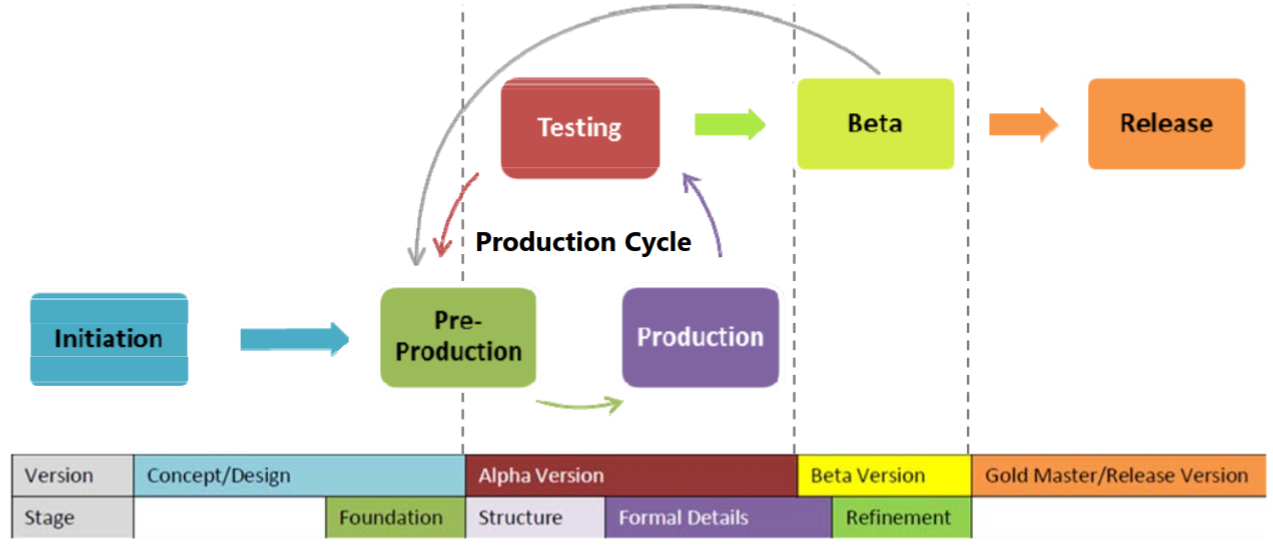
\includegraphics[scale=0.3]{img/ramadan-diagram.png}
    \caption[GDLC propuesto por Ramadan et al.]{GDLC propuesto por Ramadan et al., extraido de \textit{Game Development Life Cycle Guidelines}\cite{ramadan}}
    \label{fig:ramadan}
\end{figure}

En ese aspecto, sería interesante la aplicación de \textit{Deep Game Design}, o diseño de juego profundo. Esta es una metodología para la creación de juegos innovadores propuesta por Sebastián Blanco y Gonzalo Zabala\cite{deepdesign}. El Diseño Profundo surge a raíz de la observación de la práctica experimental de desarrolladores independientes reconocidos a nivel mundial. Este abraza la naturaleza creativa de este tipo de proyectos y permite realizar una experimentación guiada durante preproducción, pero sin llegar a ser rígida.

Blanco y Zabala hacen uso de las siguientes definiciones:

\begin{itemize}
    \item Restricciones: Similar a reglas de juego. Delimitaan el espacio de juego y pueden estar activas o no durante el mismo. Por ejemplo, el enroque en el ajedrez es una restricción.
    \item \textit{Puzzles}: Desafíos intelectuales propuestos por el diseñador que debe resolver el jugador. Siendo el videojuego un sistema, al encontrarse un \textit{puzzle} el jugador debe buscar una solución basada en ideas preconcebidas sobre el sistema e integrar nuevas ideas sobre este a través de la observación y la experimentación.
\end{itemize}

Sabiendo esto, el diseño de juego profundo se divide en tres etapas:

\begin{itemize}
    \item Definición: se expresa una idea a explorar de forma clara y concisa. Se enuncian principios de diseño, como podrían ser \textit{"fácil de aprender, difícil de dominar"} o \textit{"exploración del duelo a través de las mecánicas jugables"}. A continuación, se elabora un prototipo que represente el espacio de juego necesario para explorar la idea. Este prototipo se realiza con un conjunto atómico de reglas que se mantiene constante durante el proceso. Contiene los primeros \textit{puzzles} para validar que las ideas jugables se transmiten de forma exitosa al jugador.
    \item Exploración: se crean nuevas restricciones en el espacio de juego derivadas de las existentes de su raíz, siempre y cuando no se invaliden las anteriores. Esta relación puede representarse con una estructura jerárquica en forma de árbol de las reglas de juego. Por cada nodo, es decir cada restricción, se diseña un conjunto de \textit{puzzles} específico para transmitir al jugador la restricción ideada y verificar su internalización. De este grafo, se pueden extraer tres métricas: \textbf{profundidad}, la altura del árbol de restricciones, \textbf{complejidad}, cantidad de elementos y relaciones que el jugador debe internalizar para cumplir los objetivos, y \textbf{elegancia}, que se deriva de una menor complejidad con mayor profundidad.
    \item Finalización: el diseñador emplea su criterio para determinar qué subconjunto del árbol de restricciones y qué \textit{puzzles} se utilizarán para transmitir en el juego el diseño establecido.
\end{itemize}

Este proceso permite al diseñador adquirir una visión muy profunda y clara sobre su propio sistema, lo cual es fundamental para la redacción del GDD y el paso a producción del proyecto, ya que encauza la extensión del mismo y minimiza el riesgo a posibles cambios durante la siguiente fase.

\subsection{Problemas y riesgos comunes}

Kanode et al\cite{kanode} realizaron un estudio sobre los principales retos del desarrollo de videojuegos. Estos son algunos de ellos:

\begin{itemize}
    \item \textbf{Integración de recursos multimedia}: Recursos como las imágenes, modelos, animaciones o música son desarrollados por expertos de distintas materias en tandem con los ingenieros y programadores. Es necesario una comunicación precisa entre los distintos profesionales y desarrollar herramientas para su rápida integración en el proyecto. McKenzie et al. también menciona cómo un punto de conflicto común suele ser el choque entre la ingeniería y las disciplinas creativas.
    \item \textbf{Alcance del proyecto}: No es extraño que en videojuegos se realice una estimación pobre de el alcance del proyecto. Durante preproducción, puede parecer factible realizar cierto contenido que, durante de producción, liquidan el presupuesto. En el postmortem de \textit{Bioshock}\cite{bioshock} se cuenta cómo se estimó un desarrollo de dos años para el juego, cuando finalmente tomó tres años completarlo.
    \item \textbf{Gestión de proyectos}: Los equipos tienden a ser más grandes y más diversos. La falta de mecanismos para obtener información sobre el estado real del desarrollo impide identificar posibles problemas.
    \item \textbf{Realización pobre de GDD}: Un GDD con carencias puede avocar al equipo a perder el rumbo durante la producción. Esto se traduce en retrasos, milestones fallidas, errores y otros defectos.
\end{itemize}

Por otro lado, Schmalz et al. identifican otros tres riesgos exclusivos en videojuegos:

\begin{itemize}
    \item \textbf{Audiencia}: riesgos asociados con conectar con el público objetivo del producto y ajustar el nivel dificultad apropiado.
    \item \textbf{Fun factor}: riesgos asociados con asegurar que el juego es lo suficientemente divertido para poder ser monetizado.
    \item \textbf{Originalidad}: riesgos asociados con crear un juego lo suficientemente innovador para ser relevante en el mercado.
\end{itemize}

Petrillo et al.\cite{petrillo} añade el riesgo de \textit{feature creep}: significa una adición gradual y descontrolada de características y funcionalidades a un proyecto. Está relacionado con la mala planificación del alcance.

Todos estos riesgos y problemas tienen como última consecuencia una productividaad baja, que se traduce en no alcanzar los objetivos propuestos en preproducción. Esto suele llevar a casos como el de \textit{Bioshock} en el que se invierte más tiempo en terminar el desarrollo, pero también suele acabar con los empleados realizando horas extras para paliar la mala planificación. El \textbf{crunch} en videojuegos es el uso sistematizado de horas extra, periodos con carga de trabajo extrema en las que es común ver jornadas de 12 horas entre 6 y 7 días de la semana.

Problematicas comunes en el desarrollo:
-testing automático sensible a cambios
- Es común el uso de crunch de forma sistematizada en desarrollos

\section{Género Metroidvania}

\subsection{Contexto}

El género \textit{metroidvania} enmarca videojuegos que combinan la acción y/o plataformeo\footnote{Los videojuegos de plataformas consisten en superar obstáculos a través del movimiento de un personaje} con la exploración no lineal de un mapa interconectado. Investigando dicho mapa se suelen obtener objetos y mejoras para el personaje del jugador que le permiten abrir nuevos caminos y llegar a lugares a los que antes no podría acceder.

\begin{figure}[h]
    \centering
    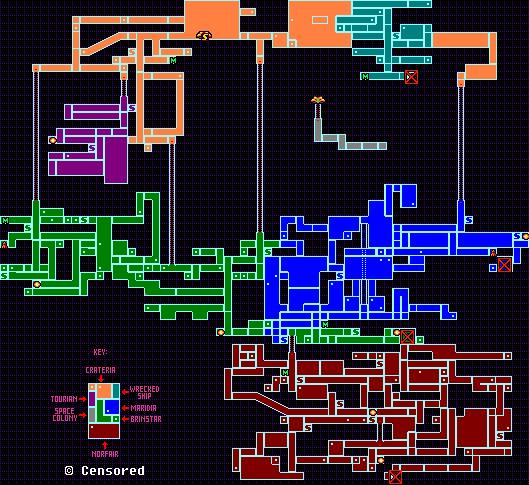
\includegraphics[scale=2.0]{img/smetrmap.jpg}
    \caption[Planos del mapa explorable en Super Metroid]{Planos del mapa explorable en Super Metroid, Nintendo 1994, extraido de \href{https://metroiddatabase.com/maps/}{Metroid Database}}.
    \label{fig:supermetroidmap}
\end{figure}

Su nombre es una combinación de las franquicias \textit{Metroid} (Nintendo, 1986) y \textit{Castlevania} (Konami, 1986), consideradas por lo general de las más influyentes del género. El término fue acuñado de forma popular, existiendo alternativas como \textit{search-action}, con un uso más extendido en Japón y usada por Nintendo en sus comunicaciones oficiales.

Aunque existen juegos anteriores que podrían definirse como metroidvanias como \textit{Below the Root}(Dale DeSharone, 1984) y \textit{Brain Braker} (Enix, 1985), se suele considerar a Metroid como quien cimienta las bases del género. En Metroid (1986) el jugador controla a Samus Aran, una cazarrecompensas espacial, con la misión de explorar unas instalaciones subterráneas del planeta Zebes y recuperar un espécimen de \textit{metroide} de las manos de unos piratas espaciales. La franquicia está influenciada por la película Alien. Esto se puede observar en su temática espacial o algunas referencias dentro del juego, como Ridley, el antagonista principal que comparte nombre con el director de cine.

La saga Castlevania relata la historia de la familia Belmont en su centenaria lucha contra el conde Drácula, el cual resucita cada 100 años. En estos juegos el jugador por lo general debe explorar el castillo de Drácula para encontrarle y derrotarle. Curiosamente, las primeras entregas no pueden considerarse metroidvanias, si no juegos de acción. No fue hasta 1997 cuando con \textit{Castlevania: Symphony of the Night} para la consola Playstation que adopraron esta nueva estructura, pero su éxito e influencia cultural fue suficiente para copresidir el nombre del género.

\subsection{Datos de mercado}

A la hora de estudiar el mercado de los juegos del género, se limitó la búsqueda a juegos lanzados para ordenador, concretamente en la plataforma de venta \href{https://store.steampowered.com/?l=spanish}{Steam}. Esto se debe a que el mercado más fácilmente accesible para desarrolladores independientes es el de ordenadores. Desarrollar y publicar en consolas suele requerir el uso de kits de desarrollo\footnote{Los kits de desarrollo son consolas especiales con funcionalidades para la depuración} usualmente distribuidas por las propias Nintendo, Microsoft o Sony, además de necesitar una aprobación más estrictas para entrar en las tiendas digitales de dichas plataformas. En cuanto al mercado del PC, Steam cuenta con más del 70\% de la cuota de mercado\cite{pc-market-share}, siendo este el estándar para comprar y jugar videojuegos.

Es difícil conocer con precisión las ventas de juegos de steam, ya que son datos que no suelen ser públicos. SteamSpy\cite{steamspy} es una web que se dedica al \textit{escrapear} la web para recopilar datos aproximados. Aunque algunos de esos datos están restringidos tras una barrera de pago, existe un estudio\cite{steamgames-genre} con datos de ventas por etiquetas hasta el año 2022.

\begin{figure}[h]
    \centering
    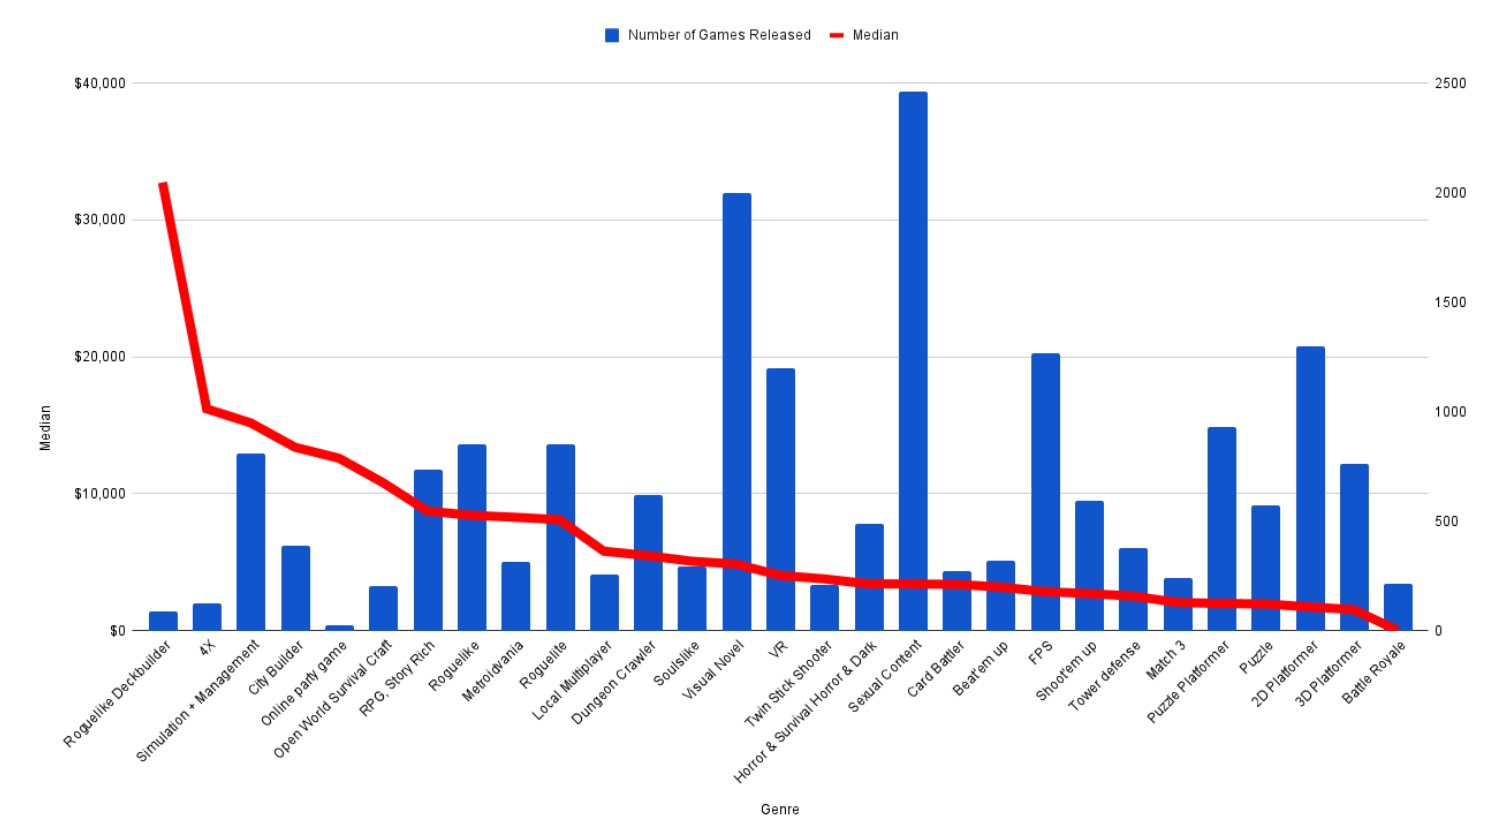
\includegraphics[scale=0.28]{img/genres-chart.png}
    \caption[Datos de venta por género en steam]{Planos del mapa explorable en Super Metroid, Nintendo 1994, extraido de \href{https://metroiddatabase.com/maps/}{Metroid Database}Número de juegos lanzados y mediana de ganancias en steam entre 2019 y 2022}.
    \label{fig:steamgenreschart}
\end{figure}

En la figura \ref{fig:steamgenreschart} se puede apreciar cómo \textit{Metroidvania} está entre las diez etiquetas con mayor mediana de ganancia. La mediana es algo menor de \$10.000, por lo que la mitad de los juegos analizados obtuvieron como mínimo esos ingresos. Se puede ver que el número de juegos no es demasiado elevado comparado con otras entradas, por lo que se puede deducir que el mercado del género no está muy saturado. Haciendo uso del buscador de SteamSpy, se puede observar que la mediana del precio de venta es de \$9.99 y el tiempo medio de juego es de 2:52 horas.

Estos datos son insuficientes para realizar una predicción real sobre cuanto podría vender el juego, pero se pueden sacar algunas conclusiones. El mercado no parece saturado y la mediana de ganancias es relativamente alta. Se tiene una aproximación del rango de precio al que se podría vender el juego, aunque esto dependerá de características concretas del mismo como su duración y la calidad percibida por el usuario. Además se tiene una estimación del tiempo que suele dedicar un usuario medio al género, dato clave para decidir la extensión del proyecto.

\subsection{Estudio del diseño}

El lector puede pensar que el diseño de videojuegos es una disciplina que no compete a la ingeniería. Si bien no es un aspecto técnico, guarda ciertos parecidos con el diseño de interfaces y la UX (\textit{user experiencie}). En una app convencional, estas dos materias se encargan de organizar los elementos del software de tal manera que el usuario lo navegue de la forma agradable y eficaz para conseguir su objetivo. El diseño en VJ actua de manera similar: cómo organizar o presentar los elementos del juego para provocar en el jugador una determinada sensación o sentimiento.

Esta disciplina es todavía joven. Aunque pueden encontrarse multitud de libros sobre el tema como \textit{Rules of Play: Game Design Fundamentals}\cite{rules-of-play} o \textit{Game Feel, a games designer guide to virtual sensation}\cite{gamefeel}, no es una disciplina asentada en la academia y no existen unos cimientos sólidos. Estos textos suelen describir una serie de principios y buenas prácticas que por lo general suelen ser útiles y deseables, pero que en última instancia dependen del contexto del juego que se vaya a desarrollar y de la intención del autor. Por ejemplo, en un juego de disparos un conviene implementar unos controles responsivos que permitan al jugador maniobrar y responder de forma ágil ante el ataque de un soldado enemigo. Pero, ¿y si es un juego de terror? En ese caso quizás sería interesante aplicar unos controles menos responsivos, más lentos, que generen más fricción, para que el jugador se vea impotente ante los monstruos que intentan darle caza.

Es difícil definir dónde empieza y dónde acaba el diseño de videojuegos, ya que puede abarcar muchas áreas. Una de ellas es el \textbf{diseño de niveles}, responsable de la organización de los espacios del juego para plantear un reto o experiencia concreta. También lo es el \textbf{diseño de sonido}, componer la \textbf{banda sonora}, la \textbf{animación}, el \textbf{guión}, el \textbf{arte}... Todas estas disciplinas condicionan la experiencia final. 

No se profundizará en todas estas disciplinas, ya que resultaría inabarcable y se prefiere centrarse en lo técnico del proyecto, pero en los próximos párrafos se repasarán cuestiones generales de diseño a la hora de abordar un metroidvania.

Se tuvieron como referencia los siguientes títulos:

\begin{itemize}
    \item Saga Metroid: Super Metrois, Metroid Zero Mission, Metroid Fusion, trilogía Metroid Prime, Samus Returns y Metroid Dread (Nintendo, Retro Studios y Mercury Steam).
    \item Hollow Knight y su secuela, Hollow Knight Silksong (Team Cherry).
    \item Axiom Verge (Thomas Happ Games).
    \item Xeodrifter (Renegade Kid).
    \item Bobo Robo (Sokpop Collective).
    \item Saga The Legend of Zelda. No pertenecen al género, pero contienen mazmorras cuyos principios de diseño son aplicables (Nintendo).
    \item Castlevania: Portrait of Ruin (Konami).
    \item Hollow Floor (Ahmed Khalifa).
    \item Gato Roboto (Doinksoft).
    \item Dead Cells (Motion Twin).
\end{itemize}

Para entender el diseño subyacente, además de analizar estos títulos, se hizo uso de \textit{Boss Keys}\cite{boss-keys}, una serie de video ensayos realizados por el divulgador Mark Brown en los que se analizan la estructura de la progresión de algunos de los juegos mencionados anteriormente.

\begin{figure}[h]
    \centering
    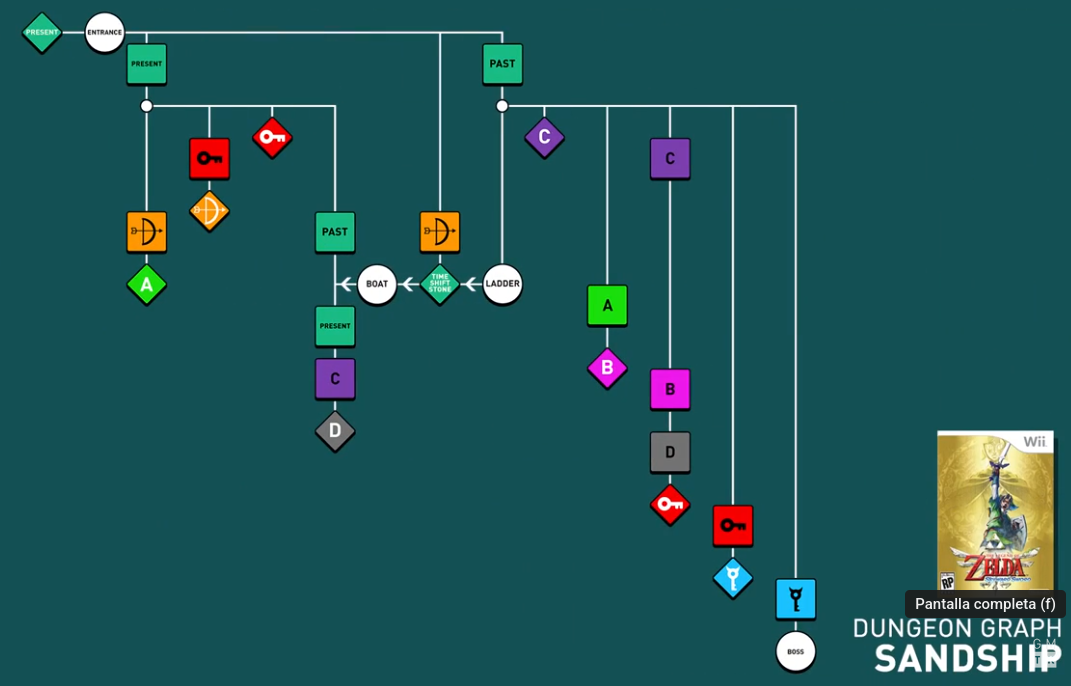
\includegraphics[scale=0.28]{img/mark-brown.png}
    \caption[Diagrama de progresión de una mazmorra de The Legend of Zelda]{Diagrama de progresión de progresión de The Legend of Zelda extraido de \href{https://www.youtube.com/@GMTK}{Game Maker's Toolkit}}.
    \label{fig:markbrown}
\end{figure}

Las conclusiones fueron los siguientes pilares sobre los que se propone que se debería construir un buen metroidvania:

\textbf{Exploración}: El núcleo jugable en todos los casos pasa por avanzar por un mapa no lineal, es decir, la exploración no consiste en ir de punto A a punto B, sino por ejemplo, ir de A a B, pero para entrar a B se necesita una llave que se consigue yendo a C. Como ejemplo se tiene el diagrama de la figura \ref{fig:markbrown}. Si se dibujara sobre el mapa el recorrido que debe hacer el jugador, debe parecerse más a las raíces de un árbol que a un circuito de carreras.


\textbf{Progresión basada en llaves y mejoras}: El jugador no puede acceder en todo momento a todos los sitios. A veces necesitará una llave para abrir una puerta, o un objeto que le permita alcanzar cierta altura a la que no llega con un salto. Se identifican entonces dos tipos de elementos para desbloquear opciones de progresión: llaves y mejoras. Las llaves son lo que parece, objetos cuyo único propósito es desbloquear un camino. Las mejoras en cambio, son cambios sustanciales a las capacidades del personaje como una mochila propulsora, unos misiles que destruyen paredes, una cuerda para atrapar objetos lejanos. Estas, además de ampliar las acciones posibles del jugador, permiten llegar a nuevos lugares.


\textbf{Tutoriales invisibles}: En muchos de los juegos analizados, no existe una guía explícita que explique cómo progresar en el juego más allá de los controles básicos. En su lugar, se usa un modelo de tutoriales basado en la experiencia. Por ejemplo, si se desea que el jugador comprenda cómo usar la recien obtenida mochila propulsora, se le conduce hasta una estancia cuya única salida esté a gran altura y no pueda salir de ahí hasta que comprenda el uso del nuevo objeto.


\textbf{\textit{Foreshadowing} mecánico}: El \textit{foreshadowing} es una técnica narrativa que consiste en adelantar a través de pistas sucesos que ocurrirán más adelante en la trama. En los metroidvania se aplica algo similar. El jugador debe identificar zonas inaccesibles o inalcanzables por antes de obtener la mejora o llave que requieran. Esto hace más orgánica la progresión, además de darle al jugador una dirección sin necesidad de hacerla explícita. Al encontrar una mejora que le permite escalar, por ejemplo, puede pensar \textit{"recuerdo pasar por un sitio demasiado alto para llegar de un salto, iré y probaré a escalarlo"}.


\textbf{Objetivos encapsulados}: El objetivo principal del juego (a nivel macroscópico) es recorrer el mapa. Mientras se avanza, el jugador se encuentra con otros objetivos más inmediatos encapsulado dentro del marco de la exploración. Un ejemplo podría ser resolver un desafío \textit{plataformero}, acabar con unos enemigos o resolver un puzle. 


\textbf{Orientación apoyada por zonas temáticas}: Es necesario dotar a las instancias con elementos distintivos y zonas visualmente reconocibles (por ejemplo, una zona de cuevas, un laboratorio, una zona con lava, un bosque, etc.). Estos ayudan al jugador a orientarse de forma orgánica sin necesidad de abrir el menú de mapa continuamente, interrumpiendo la acción.

\section{Arquitecturas y patrones}

\section{Herramientas de testing y QA}

\section{Opciones de accesibilidad}